\documentclass[a4paper,11pt]{article}
\usepackage{amsmath}
\usepackage{graphicx}
\usepackage{float}
\usepackage[utf8]{inputenc}

\title{MaS Assignment I\\
\large The Chirikov Map}
\author{Klaas Kliffen s2369494}
\date{\today}

\begin{document}

\maketitle

\section{Introduction}

The Chirikov map is an area preserving chaotic map. It is displayed in a square with 2$\pi$ as the length of the sides.

The Chirikov map is defined by the set of functions:
\begin{align} 
p_{n+1} &= p_n + K \text{ sin}[2\pi x_n] / (2*\pi)\\
x_{n+1} &= x_n + p_{n+1}
\end{align}
These are taken modulo 1, to produce the following functions:
\begin{align} 
p_{n+1} &= \{p_n + K \text{ sin}[2\pi x_n] / (2*\pi)\} \text{ mod} 1\\ 
x_{n+1} &= \{x_n + p_{n+1}\} \text{ mod} 1
\end{align}

Taking the modulo causes the Chirikov map to be displayed in a square with 1 as the length of the sides.
The functions take the parameter $K$ as a parameter. The initial conditions are defined by values of $p$ and $x$ each in $[0,1]$.

\subsection*{Initialisation}
The system is initialised by $\{x_0,p_0\} \in [0,1] \times [0,1]$

\subsection*{a) 'Orbits' in the $x$-$p$ plane for fixed $K$}
The first part of the assignment assumes a fixed value of $K = 1$ and varies the initial conditions. The aim of this part will be to distinguish between different kinds of 'orbits'.

\subsection*{b) Behaviour for different values of $K$}
The second part will use the orbits from the first part and will use a varying value for $K$.
The aim of this part will be to explore the changing orbits for an increasing value of $K$

\section{Methods}
This section globally describes the adapted functions used in this assignment.

\subsection*{a) 'Orbits' in the $x$-$p$ plane for fixed $K$}
To generate the values describing the orbit, a step function is created to accept 2 coordinates and calculates the next coordinates from the equations 3 and 4.
This function can be used to explore the different kind of orbits given the initial values.\\
For each initial value, the first thousand iterations are run. To determine the order in which points are visited, another number of iterations may be given. These will be noted in the result section.\\

\subsection*{b) Behaviour for different values of $K$}
To plot multiple orbits for a given $K$, the step function is called multiple times, each with different pseudo-random initial values. The calculated values are then stored in two arrays to be plotted.\\
For each value of K, 50 orbits are calculated with pseudo random initial conditions, each with 1000 iterations.

\section{Results}
\subsection{a) 'Orbits' in the $x$-$p$ plane for fixed $K$}
There are three types of orbits that can be found. These will be addressed each in its own section.
\subsubsection{Points}
Barely visible are two single points in figure \ref{pointorbit} at $(0,0.5)$ and $(0.5,0.5)$. From figure \ref{pointval} it is clear that $p$ stays constant, with $x$ switching between the two points. The value of $p$ is constant, because in formula (3) the sinus component is constant with $x$ varying between two values: 0 and 0.5, both yielding a zero value for the sinus. Since $p$ is constant at 0.5, from formula (4), it is clear that x with initial condition 0.5, can only be 0 and 0.5 in an alternating order. Therefor, only 20 iterations are shown in figure \ref{pointval}.
\begin{figure}[H]
\centering
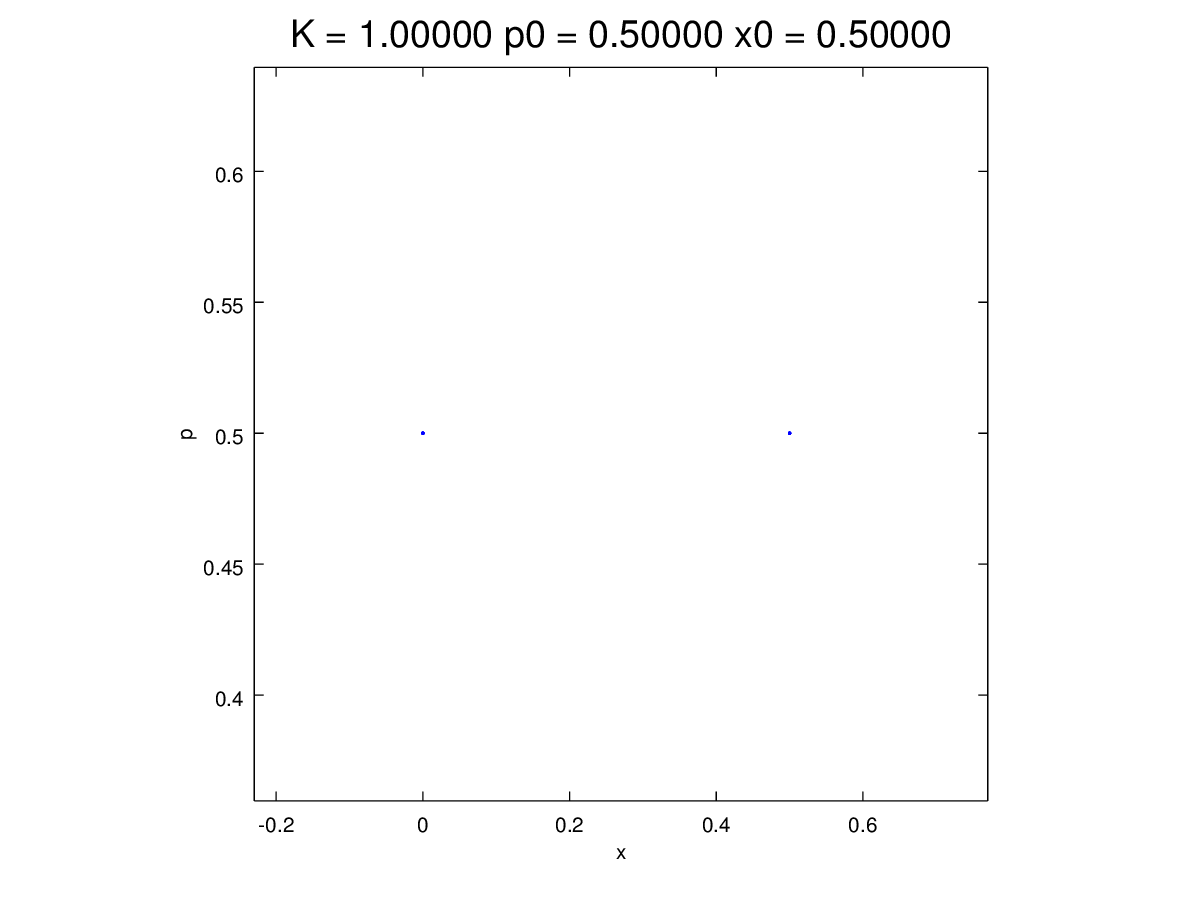
\includegraphics[width=.9\textwidth]{img/orbitpoint.png}
\caption{Orbit plot of two points}
\label{pointorbit}
\end{figure}
\begin{figure}[H]
\centering
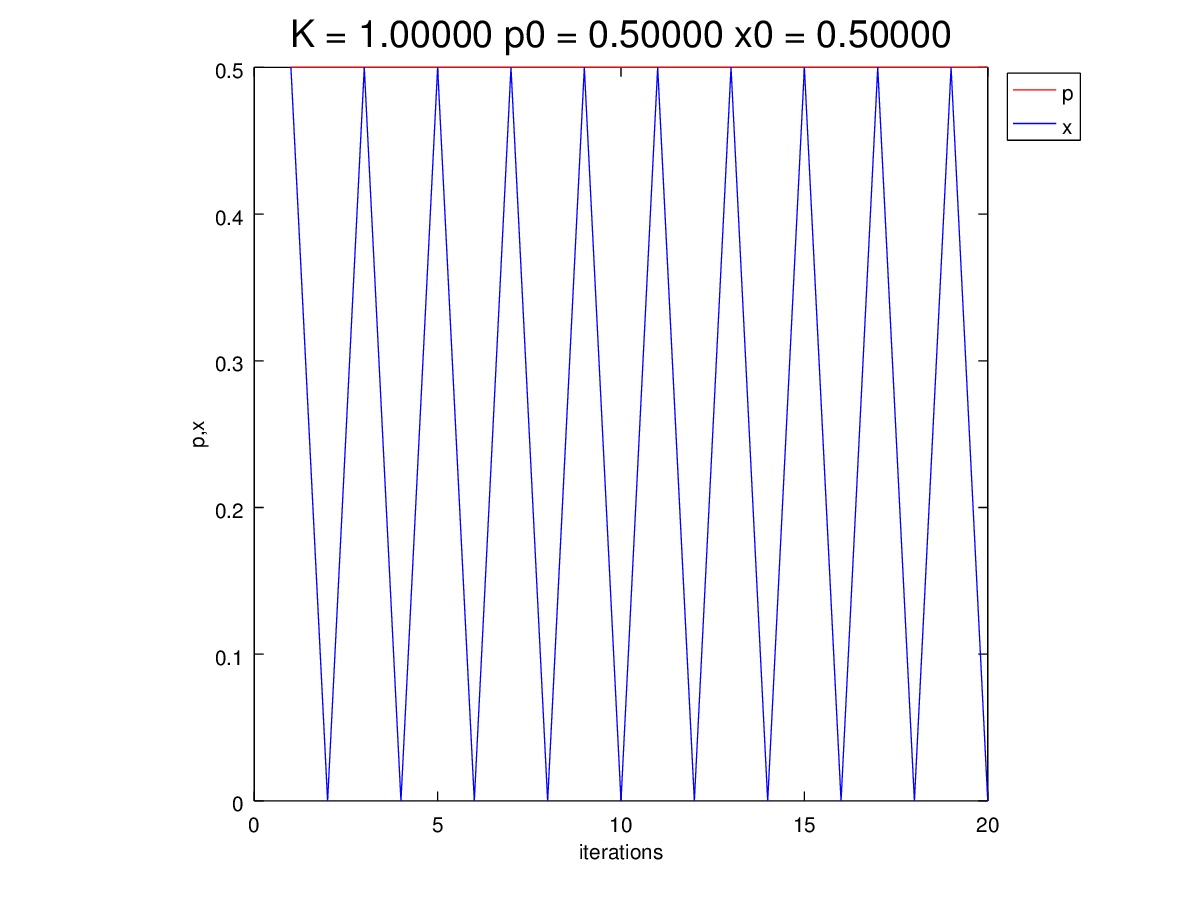
\includegraphics[width=.9\textwidth]{img/valuepoint.png}
\caption{The values for $p$ and $x$ in the first 20 iterations}
\label{pointval}
\end{figure}

\subsubsection{Curves}
\begin{figure}[H]
\centering
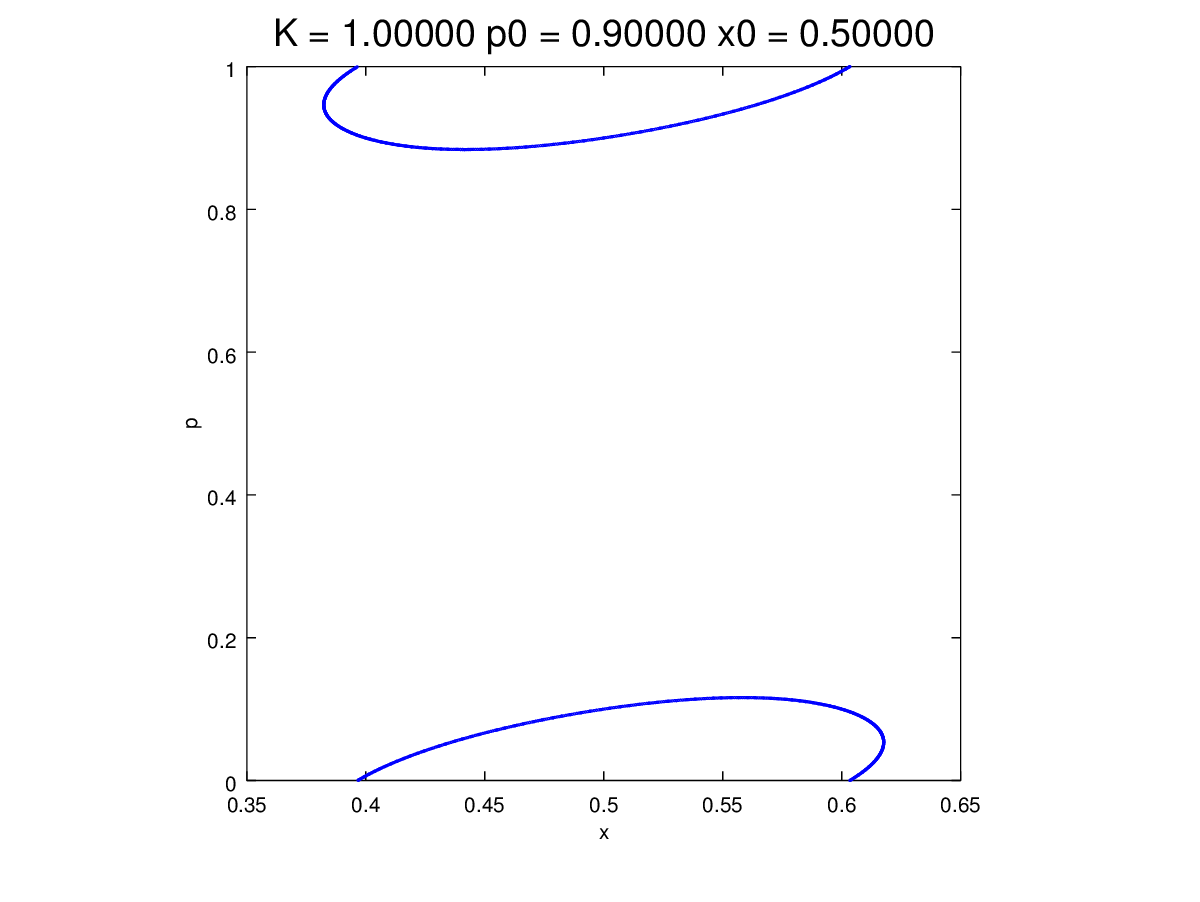
\includegraphics[width=.9\textwidth]{img/orbitcurve.png}
\caption{Orbit plot of four curves}
\label{curveorbit}
\end{figure}
\begin{figure}[H]
\centering
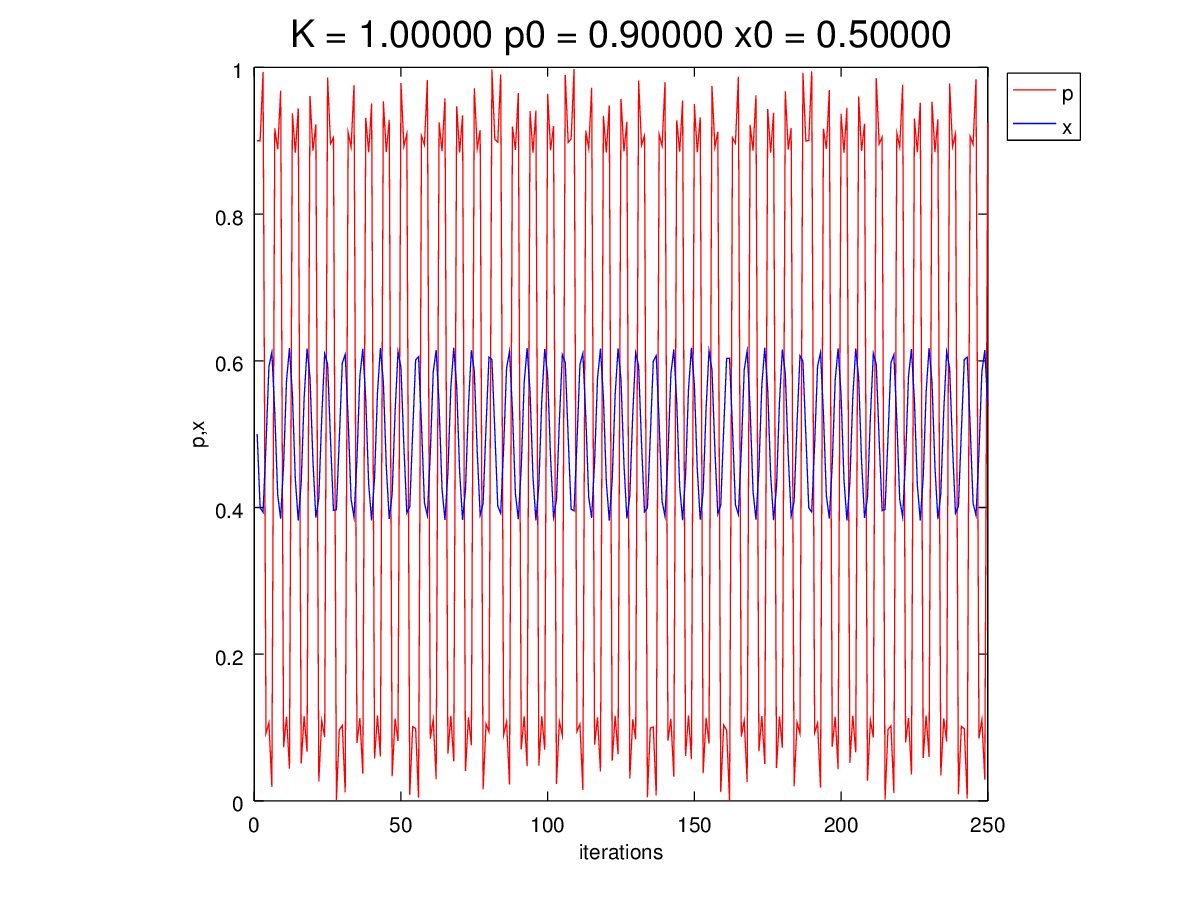
\includegraphics[width=.9\textwidth]{img/valuecurve.png}
\caption{The values for $p$ and $x$ in the first 250 iterations }
\label{curveval}
\end{figure}

\newpage

Figure \ref{curveorbit} represent curves. These curves are closed and symmetrical.The values of $p$ are in two ranges: a higher range, yielding the top curve and a lower range, yielding the lower curve. The value of $x$ varies in one range. In figure \ref{curveval} it can be seen that $x$ varies between two peaks. The curves are visited in a fixed order as figure \ref{curveval} shows for the first 250 iterations. The top curve is visited first with a few iterations. After that, the bottom curve is visited with with a similar amount of iterations.

\subsubsection{Areas}
In figure \ref{areaorbit} two dotted areas can be seen. One on the top layer and one on the bottom. These areas seem to be symmetrical around the centre point of the image. These areas seem to be filled with chaotic values. In figure \ref{areaval} the values for $p$ seem to be on the lower half of the image, but after about 300 iterations, these values seem to spike to the upper half of the image. The values for $x$ seem to be chaotic and spread about all of the $[0,1]$ range.

\begin{figure}[H]
\centering
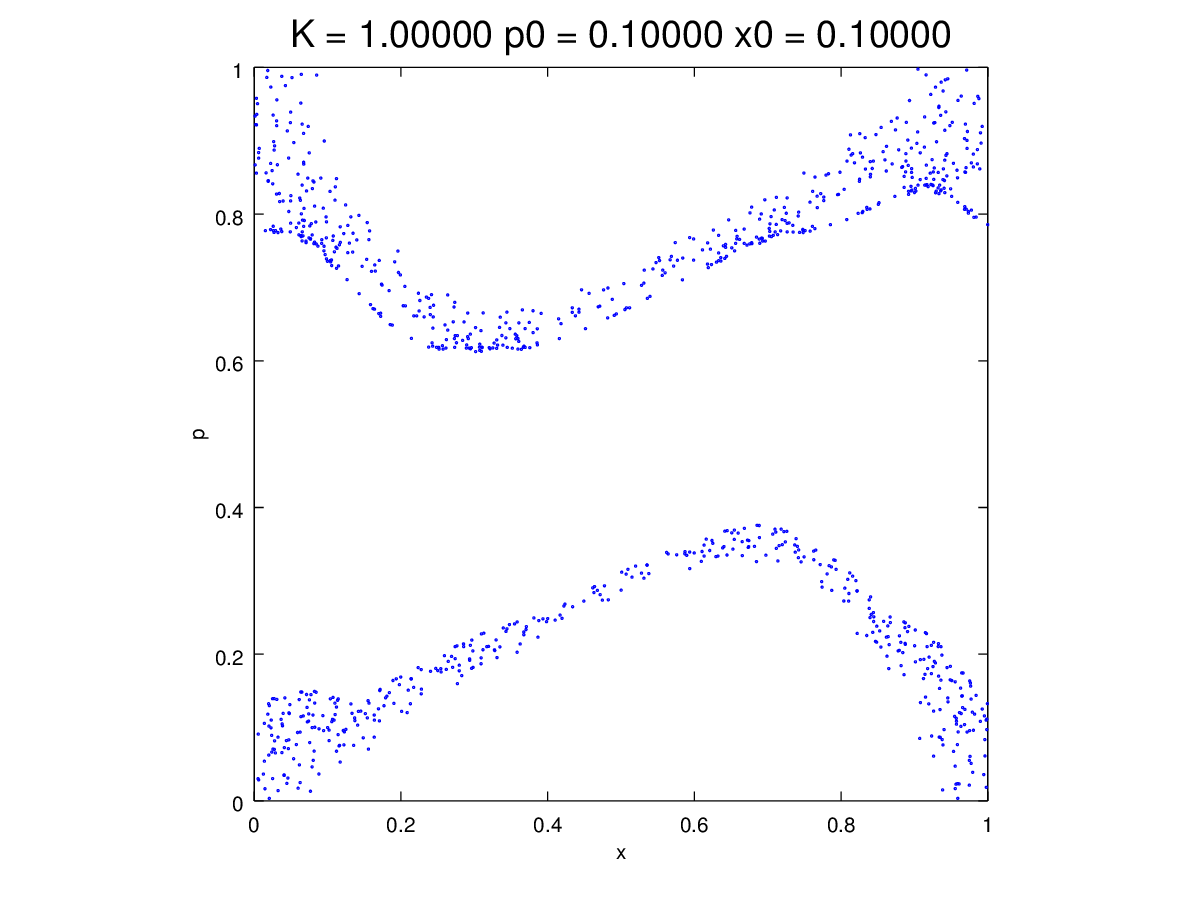
\includegraphics[width=.9\textwidth]{img/orbitarea.png}
\caption{Orbit plot of two areas}
\label{areaorbit}
\end{figure}

\newpage
\begin{figure}[H]
\centering
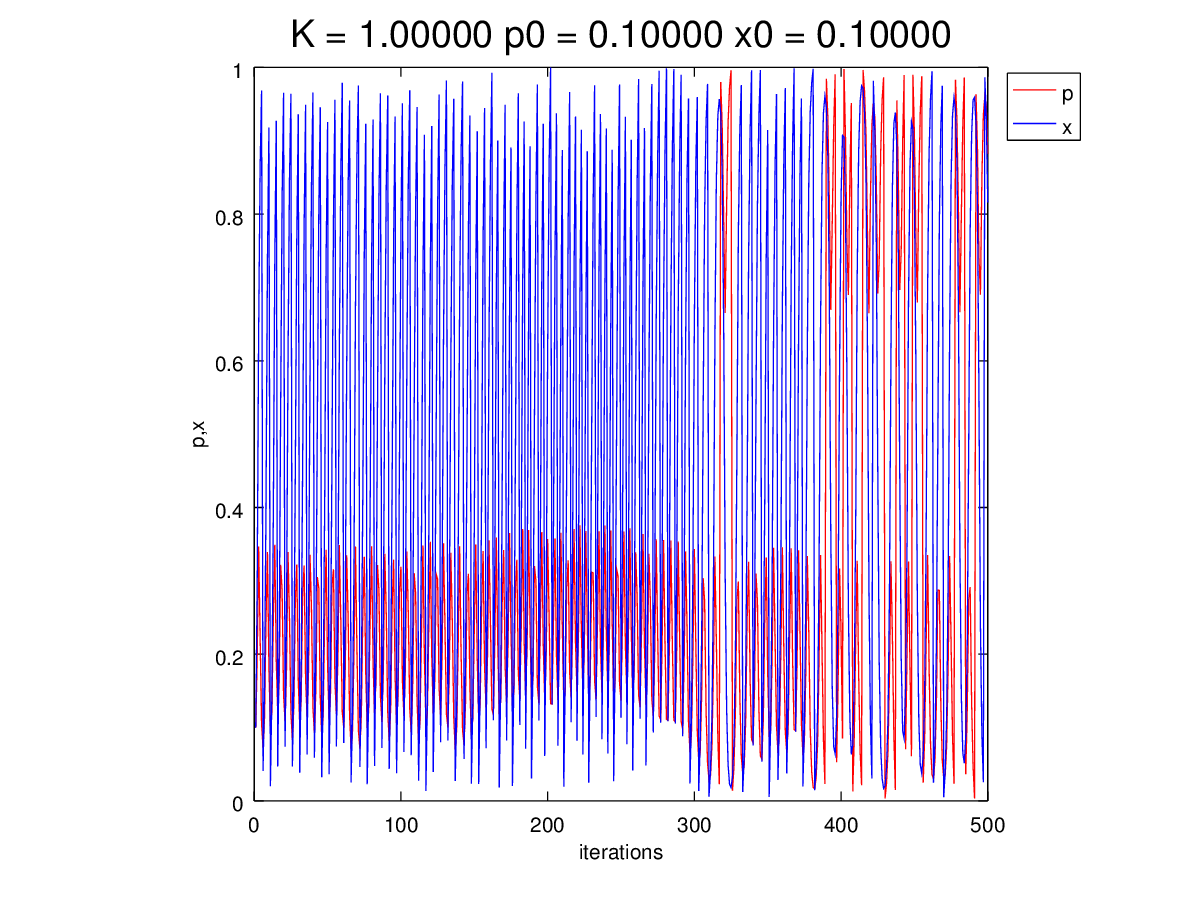
\includegraphics[width=.9\textwidth]{img/valuearea.png}
\caption{The values for $p$ and $x$ in the first 500 iterations}
\label{areaval}
\end{figure}

\subsection{b) Behaviour for different values of $K$}

The figures 7 to 22 are taken at different values for $K$ in an increasing order.

\subsubsection{Increasing value of $K$}

\begin{figure}[H]
\centering
\begin{minipage}{0.5\textwidth}
\centering
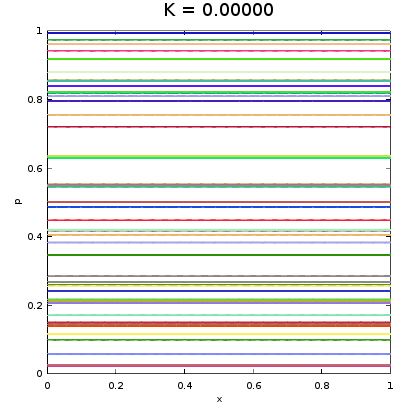
\includegraphics[width=\textwidth]{img/k0.png}
\caption{Orbits for $K = 0$}
\end{minipage}\hfill
\begin{minipage}{0.5\textwidth}
\centering
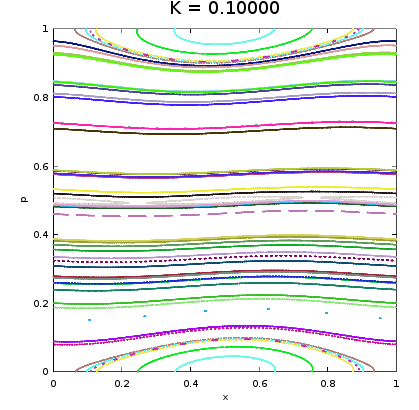
\includegraphics[width=\textwidth]{img/k01.png}
\caption{Orbits for $K = 0.1$}
\end{minipage}
\end{figure}

For value $K=0$ the orbits are plotted in figure 7. These are all horizontal lines. Since the sinus component form formula (3) is completely neglected, this value is constant. The value for $x$ however, could be anywhere in the range of [0,1]. This yields horizontal lines.

\begin{figure}[H]
\centering
\begin{minipage}{0.5\textwidth}
\centering
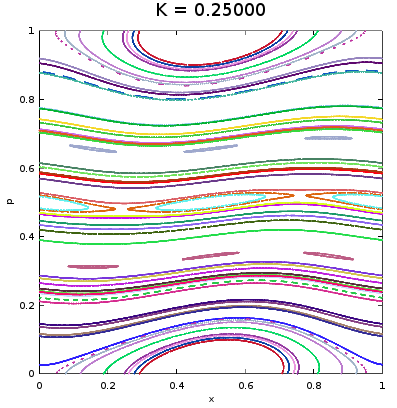
\includegraphics[width=\textwidth]{img/k025.png}
\caption{Orbits for $K = 0.25$}
\end{minipage}\hfill
\begin{minipage}{0.5\textwidth}
\centering
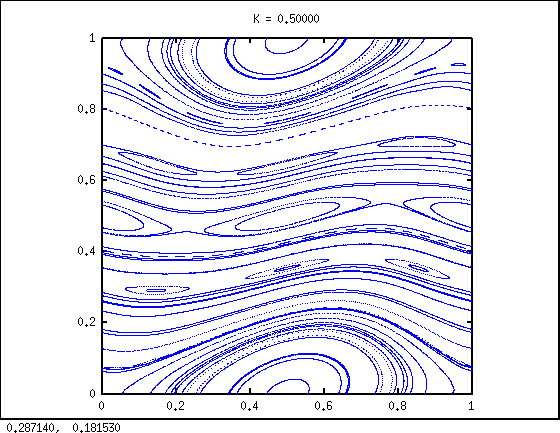
\includegraphics[width=\textwidth]{img/k05.png}
\caption{Orbits for $K = 0.5$}
\end{minipage}
\end{figure}

\begin{figure}[H]
\centering
\begin{minipage}{0.5\textwidth}
\centering
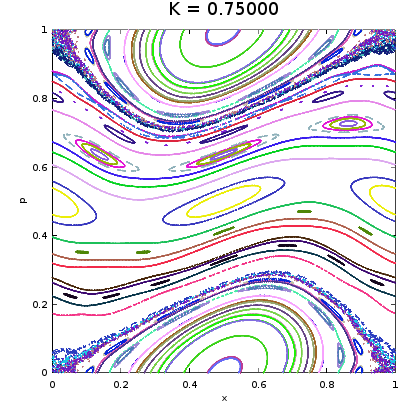
\includegraphics[width=\textwidth]{img/k075.png}
\caption{Orbits for $K = 0.75$}
\end{minipage}\hfill
\begin{minipage}{0.5\textwidth}
\centering
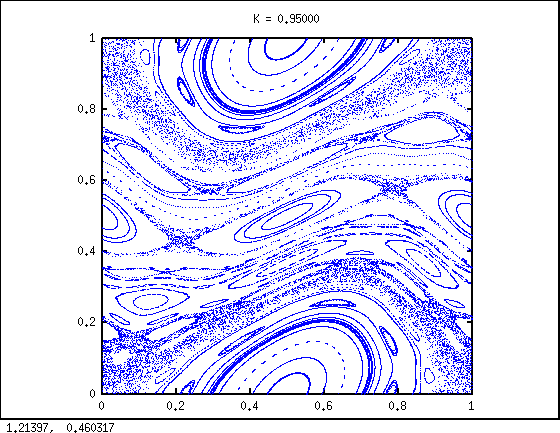
\includegraphics[width=\textwidth]{img/k095.png}
\caption{Orbits for $K = 0.95$}
\end{minipage}
\end{figure}

\begin{figure}[H]
\centering
\begin{minipage}{0.5\textwidth}
\centering
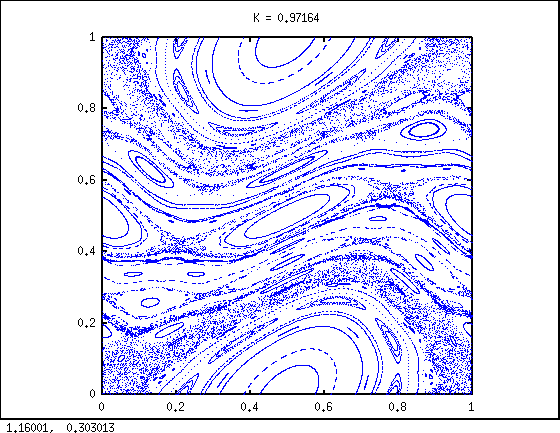
\includegraphics[width=\textwidth]{img/kc.png}
\caption{Orbits for $K_c = 0.97164$}
\end{minipage}\hfill
\begin{minipage}{0.5\textwidth}
\centering
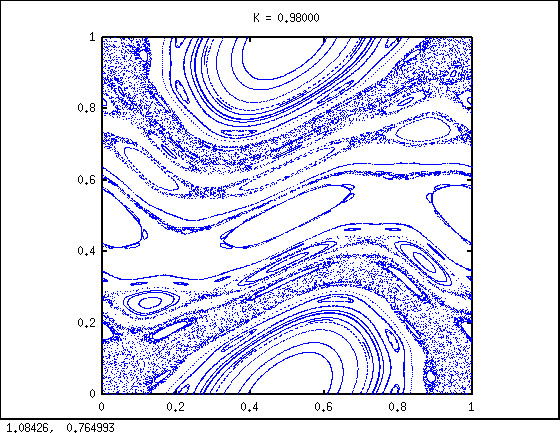
\includegraphics[width=\textwidth]{img/k098.png}
\caption{Orbits for $K = 0.98$}
\end{minipage}
\end{figure}

\begin{figure}[H]
\centering
\begin{minipage}{0.5\textwidth}
\centering
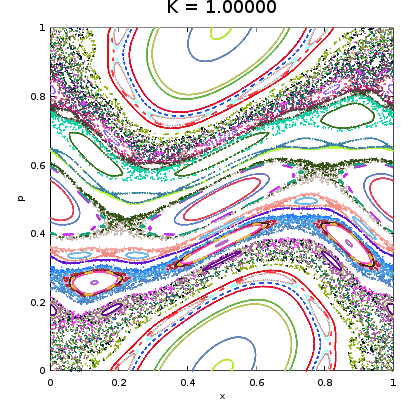
\includegraphics[width=\textwidth]{img/k1.png}
\caption{Orbits for $K = 1.0$}
\end{minipage}\hfill
\begin{minipage}{0.5\textwidth}
\centering
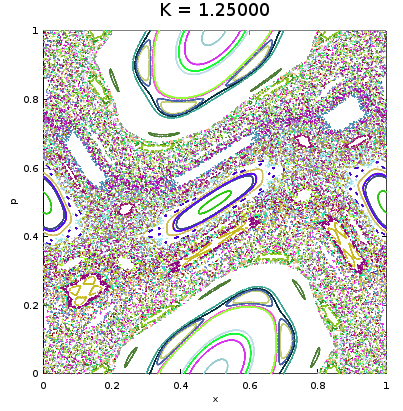
\includegraphics[width=\textwidth]{img/k125.png}
\caption{Orbits for $K = 1.25$}
\end{minipage}
\end{figure}

\begin{figure}[H]
\centering
\begin{minipage}{0.5\textwidth}
\centering
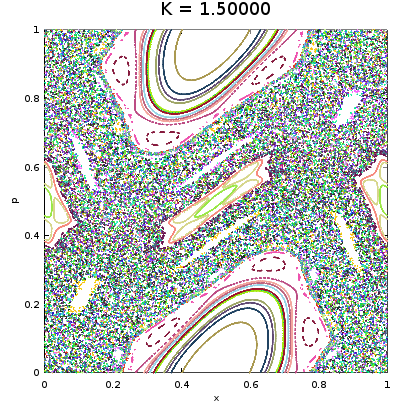
\includegraphics[width=\textwidth]{img/k15.png}
\caption{Orbits for $K = 1.5$}
\end{minipage}\hfill
\begin{minipage}{0.5\textwidth}
\centering
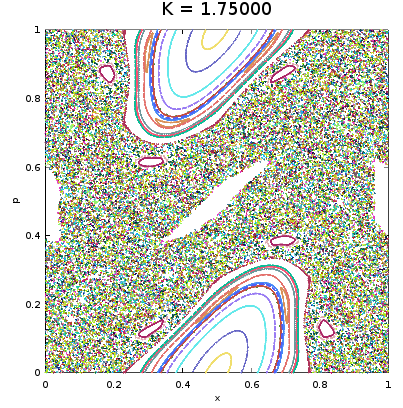
\includegraphics[width=\textwidth]{img/k175.png}
\caption{Orbits for $K = 1.75$}
\end{minipage}
\end{figure}

\begin{figure}[H]
\centering
\begin{minipage}{0.5\textwidth}
\centering
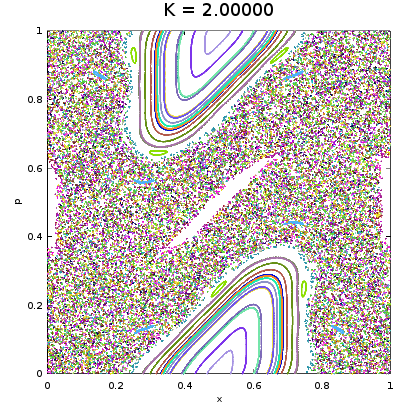
\includegraphics[width=\textwidth]{img/k2.png}
\caption{Orbits for $K = 2.0$}
\end{minipage}\hfill
\begin{minipage}{0.5\textwidth}
\centering
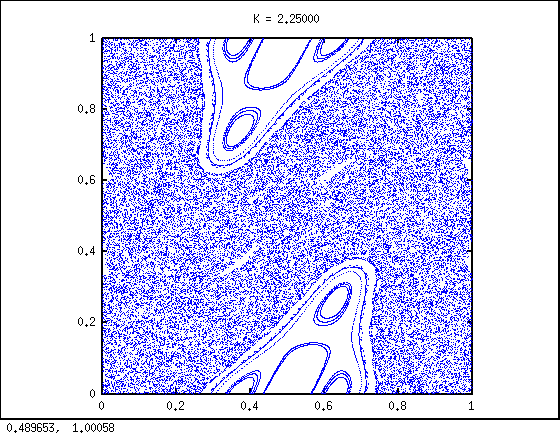
\includegraphics[width=\textwidth]{img/k225.png}
\caption{Orbits for $K = 2.25$}
\end{minipage}
\end{figure}

\begin{figure}[H]
\centering
\begin{minipage}{0.5\textwidth}
\centering
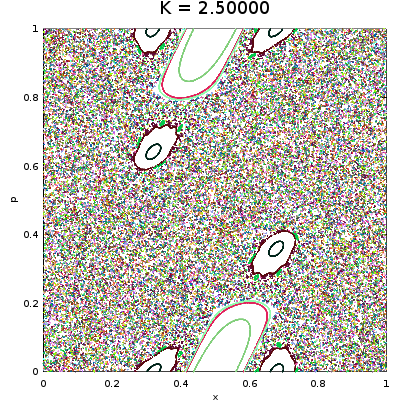
\includegraphics[width=\textwidth]{img/k25.png}
\caption{Orbits for $K = 2.5$}
\end{minipage}\hfill
\begin{minipage}{0.5\textwidth}
\centering
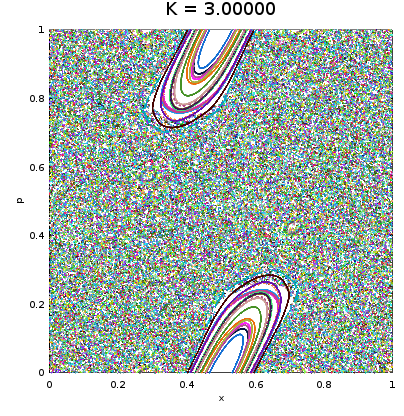
\includegraphics[width=\textwidth]{img/k3.png}
\caption{Orbits for $K = 3.0$}
\end{minipage}
\end{figure}

In figures 8 to 12 ($K$ values in the range of [0.1,0.95]) it can be seen that the straight lines at $K = 0$ slowly curve into two curves at the horizontal centre of the image. In between are similar structures of curves visible.

Above  $K = 0.75$ areas of chaotic dots appear and take up most of the image after $K = 2$, destroying the curves in the centre of the image.
After values of 3.0 for $K$ most of the area of the image is taken up by the chaotic region.\\

Around $K = 1.25$ six smaller curves can be seen on the edges of the two large curves on the top and the bottom of the image. These become bigger and move outwards away from the centre of the large curve. When $K$ reaches a value of 2.0, these satellite curves are dissolved into the chaotic region of the image. This behaviour seems similar to the period doubling of the logistic map. For values of $K$ between 2.25 and 3.0, another instance of these smaller curves can be seen.

\subsubsection{KAM orbits}
KAM orbits are orbits spanning the entire range of [0,1]. These only exist below a certain threshold value for $K$ called $K_c$. The value 0.971635 as described by Greene\cite{kval} is used as the value for $K_c$. Figures 12 to 15 show plots of orbits for values of $K$ between 0.95 and 1.0. Although figures 14 and 15 show orbits spanning the entire range of $[0,1]$, when zooming in, it becomes clear these do not follow a closed curve and are more of a chain of curves.

\section{Conclusion and discussion}

\subsection{a) 'Orbits' in the $x$-$p$ plane for fixed $K$}
From the different initial conditions three types of 'orbits' can be determined: Points, curves and areas. Each of these types has a certain order in which points are visited. For point orbits, these are clearly defined. For curves both values will vary in between ranges. For areas, the $x$ value will vary over the complete interval of $[0,1]$ and $p$ will vary only over smaller ranges.

\subsection{b) Behaviour for different values of $K$}
For an increasing value of $K$ the amount of chaotic regions will increase. For values up to $K = 0.9$ the regions will be very small to non existent. After that the regions will grow. For values of $K$ in between $[1.0,1.75]$ and $[2.0,3.0]$ there will be a process similar to period doubling with smaller curves moving outward of the large centre curve. After $K = 3.0$ the image will only consist of the centre two curves and a chaotic region.\\
Exploring the limit of KAM orbits around the value of $K_c = 0.971635$ did not lead to observable results. Possibly to issues with the resolution of the plot and the amount of points per orbit plotted.

\subsection{Discussion}
The resolution on the images is limited. It is hard to prove from figures alone that a line could cross the entire horizontal scale of an image and not be distorted by a chaotic region. Depending on the resolution and the amount of points generated for each orbit, the image yield a better view of KAM orbits.

\begin{thebibliography}{1337}
\bibitem{kval}
Greene, John M.\\
\emph{A method for determining a stochastic transition}\\
Journal of Mathematical Physics, 20, 1183-1201 (1979)\\ DOI:http://dx.doi.org/10.1063/1.524170

\end{thebibliography}
\end{document}
